\documentclass[]{book}
\usepackage{lmodern}
\usepackage{amssymb,amsmath}
\usepackage{ifxetex,ifluatex}
\usepackage{fixltx2e} % provides \textsubscript
\ifnum 0\ifxetex 1\fi\ifluatex 1\fi=0 % if pdftex
  \usepackage[T1]{fontenc}
  \usepackage[utf8]{inputenc}
\else % if luatex or xelatex
  \ifxetex
    \usepackage{mathspec}
  \else
    \usepackage{fontspec}
  \fi
  \defaultfontfeatures{Ligatures=TeX,Scale=MatchLowercase}
\fi
% use upquote if available, for straight quotes in verbatim environments
\IfFileExists{upquote.sty}{\usepackage{upquote}}{}
% use microtype if available
\IfFileExists{microtype.sty}{%
\usepackage{microtype}
\UseMicrotypeSet[protrusion]{basicmath} % disable protrusion for tt fonts
}{}
\usepackage{hyperref}
\hypersetup{unicode=true,
            pdftitle={Informatics team manual of procedures},
            pdfauthor={Ania Tassinari},
            pdfborder={0 0 0},
            breaklinks=true}
\urlstyle{same}  % don't use monospace font for urls
\usepackage{natbib}
\bibliographystyle{apalike}
\usepackage{color}
\usepackage{fancyvrb}
\newcommand{\VerbBar}{|}
\newcommand{\VERB}{\Verb[commandchars=\\\{\}]}
\DefineVerbatimEnvironment{Highlighting}{Verbatim}{commandchars=\\\{\}}
% Add ',fontsize=\small' for more characters per line
\usepackage{framed}
\definecolor{shadecolor}{RGB}{248,248,248}
\newenvironment{Shaded}{\begin{snugshade}}{\end{snugshade}}
\newcommand{\AlertTok}[1]{\textcolor[rgb]{0.94,0.16,0.16}{#1}}
\newcommand{\AnnotationTok}[1]{\textcolor[rgb]{0.56,0.35,0.01}{\textbf{\textit{#1}}}}
\newcommand{\AttributeTok}[1]{\textcolor[rgb]{0.77,0.63,0.00}{#1}}
\newcommand{\BaseNTok}[1]{\textcolor[rgb]{0.00,0.00,0.81}{#1}}
\newcommand{\BuiltInTok}[1]{#1}
\newcommand{\CharTok}[1]{\textcolor[rgb]{0.31,0.60,0.02}{#1}}
\newcommand{\CommentTok}[1]{\textcolor[rgb]{0.56,0.35,0.01}{\textit{#1}}}
\newcommand{\CommentVarTok}[1]{\textcolor[rgb]{0.56,0.35,0.01}{\textbf{\textit{#1}}}}
\newcommand{\ConstantTok}[1]{\textcolor[rgb]{0.00,0.00,0.00}{#1}}
\newcommand{\ControlFlowTok}[1]{\textcolor[rgb]{0.13,0.29,0.53}{\textbf{#1}}}
\newcommand{\DataTypeTok}[1]{\textcolor[rgb]{0.13,0.29,0.53}{#1}}
\newcommand{\DecValTok}[1]{\textcolor[rgb]{0.00,0.00,0.81}{#1}}
\newcommand{\DocumentationTok}[1]{\textcolor[rgb]{0.56,0.35,0.01}{\textbf{\textit{#1}}}}
\newcommand{\ErrorTok}[1]{\textcolor[rgb]{0.64,0.00,0.00}{\textbf{#1}}}
\newcommand{\ExtensionTok}[1]{#1}
\newcommand{\FloatTok}[1]{\textcolor[rgb]{0.00,0.00,0.81}{#1}}
\newcommand{\FunctionTok}[1]{\textcolor[rgb]{0.00,0.00,0.00}{#1}}
\newcommand{\ImportTok}[1]{#1}
\newcommand{\InformationTok}[1]{\textcolor[rgb]{0.56,0.35,0.01}{\textbf{\textit{#1}}}}
\newcommand{\KeywordTok}[1]{\textcolor[rgb]{0.13,0.29,0.53}{\textbf{#1}}}
\newcommand{\NormalTok}[1]{#1}
\newcommand{\OperatorTok}[1]{\textcolor[rgb]{0.81,0.36,0.00}{\textbf{#1}}}
\newcommand{\OtherTok}[1]{\textcolor[rgb]{0.56,0.35,0.01}{#1}}
\newcommand{\PreprocessorTok}[1]{\textcolor[rgb]{0.56,0.35,0.01}{\textit{#1}}}
\newcommand{\RegionMarkerTok}[1]{#1}
\newcommand{\SpecialCharTok}[1]{\textcolor[rgb]{0.00,0.00,0.00}{#1}}
\newcommand{\SpecialStringTok}[1]{\textcolor[rgb]{0.31,0.60,0.02}{#1}}
\newcommand{\StringTok}[1]{\textcolor[rgb]{0.31,0.60,0.02}{#1}}
\newcommand{\VariableTok}[1]{\textcolor[rgb]{0.00,0.00,0.00}{#1}}
\newcommand{\VerbatimStringTok}[1]{\textcolor[rgb]{0.31,0.60,0.02}{#1}}
\newcommand{\WarningTok}[1]{\textcolor[rgb]{0.56,0.35,0.01}{\textbf{\textit{#1}}}}
\usepackage{longtable,booktabs}
\usepackage{graphicx,grffile}
\makeatletter
\def\maxwidth{\ifdim\Gin@nat@width>\linewidth\linewidth\else\Gin@nat@width\fi}
\def\maxheight{\ifdim\Gin@nat@height>\textheight\textheight\else\Gin@nat@height\fi}
\makeatother
% Scale images if necessary, so that they will not overflow the page
% margins by default, and it is still possible to overwrite the defaults
% using explicit options in \includegraphics[width, height, ...]{}
\setkeys{Gin}{width=\maxwidth,height=\maxheight,keepaspectratio}
\IfFileExists{parskip.sty}{%
\usepackage{parskip}
}{% else
\setlength{\parindent}{0pt}
\setlength{\parskip}{6pt plus 2pt minus 1pt}
}
\setlength{\emergencystretch}{3em}  % prevent overfull lines
\providecommand{\tightlist}{%
  \setlength{\itemsep}{0pt}\setlength{\parskip}{0pt}}
\setcounter{secnumdepth}{5}
% Redefines (sub)paragraphs to behave more like sections
\ifx\paragraph\undefined\else
\let\oldparagraph\paragraph
\renewcommand{\paragraph}[1]{\oldparagraph{#1}\mbox{}}
\fi
\ifx\subparagraph\undefined\else
\let\oldsubparagraph\subparagraph
\renewcommand{\subparagraph}[1]{\oldsubparagraph{#1}\mbox{}}
\fi

%%% Use protect on footnotes to avoid problems with footnotes in titles
\let\rmarkdownfootnote\footnote%
\def\footnote{\protect\rmarkdownfootnote}

%%% Change title format to be more compact
\usepackage{titling}

% Create subtitle command for use in maketitle
\providecommand{\subtitle}[1]{
  \posttitle{
    \begin{center}\large#1\end{center}
    }
}

\setlength{\droptitle}{-2em}

  \title{Informatics team manual of procedures}
    \pretitle{\vspace{\droptitle}\centering\huge}
  \posttitle{\par}
    \author{Ania Tassinari}
    \preauthor{\centering\large\emph}
  \postauthor{\par}
      \predate{\centering\large\emph}
  \postdate{\par}
    \date{2019-06-25}

\usepackage{booktabs}
\usepackage{amsthm}
\makeatletter
\def\thm@space@setup{%
  \thm@preskip=8pt plus 2pt minus 4pt
  \thm@postskip=\thm@preskip
}
\makeatother

\begin{document}
\maketitle

{
\setcounter{tocdepth}{1}
\tableofcontents
}
\hypertarget{about}{%
\chapter{About}\label{about}}

This is a manual of operations for the Agios Informatics team. Its puspose is to:

\begin{itemize}
\tightlist
\item
  provide a resource on \textbf{best practices} (Chapter \ref{bestpractices})
\item
  aid in setting up effective and reproducible \textbf{project workflows} (Chapter \ref{workflows})
\item
  promote learning and sharing of \textbf{ideas} (Chapter \ref{toolbox}).
\end{itemize}

\hypertarget{bestpractices}{%
\chapter{Best practices}\label{bestpractices}}

\hypertarget{reproducible-research}{%
\section{Reproducible research}\label{reproducible-research}}

\hypertarget{purpose}{%
\subsection{Purpose}\label{purpose}}

\begin{enumerate}
\def\labelenumi{\arabic{enumi}.}
\tightlist
\item
  Improve collaborative analyses:
\end{enumerate}

\begin{itemize}
\tightlist
\item
  make sharing easier
\item
  enable retrieval and interpretation of results long after analysis ended
\end{itemize}

\begin{enumerate}
\def\labelenumi{\arabic{enumi}.}
\setcounter{enumi}{1}
\item
  Simplify hand-off to Biostats
\item
  Improve confidence in our data and results
\end{enumerate}

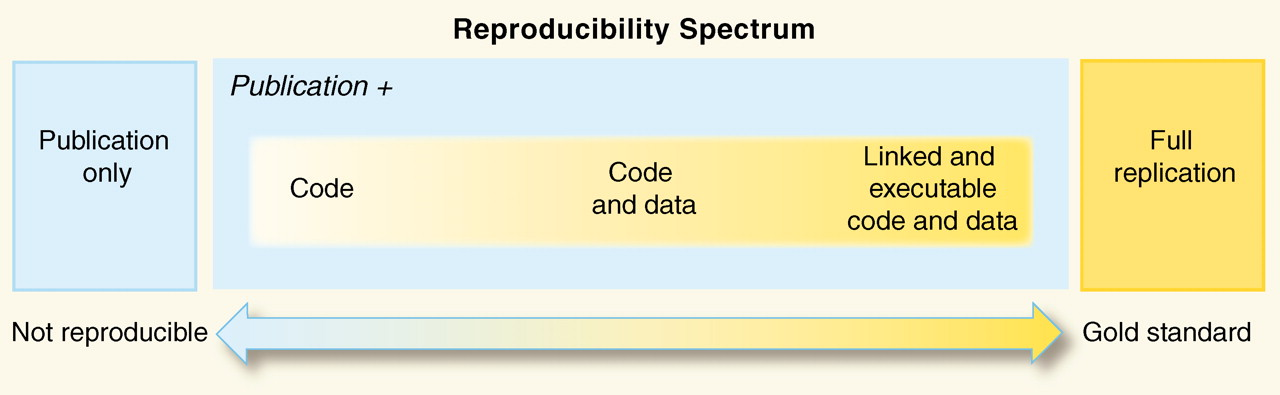
\includegraphics{images/reprodresearch.jpg}

Source: Peng et al., \emph{Reproducible Research in Computational Science}. Science 2011.

\hypertarget{dos-and-donts-of-reproducible-research}{%
\subsection{DO's and DON'T's of reproducible research}\label{dos-and-donts-of-reproducible-research}}

{DO} start with good science
{DON'T} do things by hand
Was any part of this analysis done by hand?
- If so, are those parts precisely documented?
- Does the documentation match reality?
{DON'T} point and click
{DO} teach a computer
{DO} use version control
{DO} keep track of your software environment
{DON'T} save any output (until it's time to write a paper)
{DO} set your seed

Source: Reproducible Research at Coursera

\hypertarget{version-control}{%
\section{Version control}\label{version-control}}

\hypertarget{code-guidelines}{%
\section{Code guidelines}\label{code-guidelines}}

\hypertarget{r}{%
\subsection{R}\label{r}}

\begin{itemize}
\tightlist
\item
  \href{https://style.tidyverse.org}{Tidyverse Style Guide}
\item
  \href{https://google.github.io/styleguide/Rguide.xml}{Google's R Style Guide}
\end{itemize}

\hypertarget{workflows}{%
\chapter{Project workflows}\label{workflows}}

\hypertarget{using-workflowr}{%
\section{Using Workflowr}\label{using-workflowr}}

\hypertarget{quick-start}{%
\subsection{Quick Start}\label{quick-start}}

This is a quick version of everything listed below, if you want more clear or specfic instructions then please skip this chaper and follow the steps in the following one.

\hypertarget{set-up}{%
\subsubsection{Set Up}\label{set-up}}

In the \texttt{Console} tab of RStudio in \texttt{(None)} project:

\begin{Shaded}
\begin{Highlighting}[]
\KeywordTok{install.packages}\NormalTok{(}\StringTok{"workflowr"}\NormalTok{)}
\KeywordTok{library}\NormalTok{(}\StringTok{"workflowr"}\NormalTok{)}
\KeywordTok{wflow_git_config}\NormalTok{(}\DataTypeTok{user.name =} \StringTok{"First Last"}\NormalTok{, }\DataTypeTok{user.email =} \StringTok{"first.last@agios.com"}\NormalTok{)}
\end{Highlighting}
\end{Shaded}

\hypertarget{creating-projects}{%
\subsubsection{Creating Projects}\label{creating-projects}}

In the \texttt{Console} tab,

\begin{Shaded}
\begin{Highlighting}[]
\KeywordTok{wflow_start}\NormalTok{(}\StringTok{"PROJECT_NAME"}\NormalTok{)}
\KeywordTok{wflow_build}\NormalTok{()}
\KeywordTok{wflow_publish}\NormalTok{(}\KeywordTok{c}\NormalTok{(}\StringTok{"analysis/*.Rmd"}\NormalTok{), }\StringTok{"Publish the initial files for PROJECT_NAME"}\NormalTok{)}
\end{Highlighting}
\end{Shaded}

\hypertarget{connecting-to-gitlab}{%
\subsubsection{Connecting to GitLab}\label{connecting-to-gitlab}}

In the \texttt{Console} tab,

\begin{Shaded}
\begin{Highlighting}[]
\KeywordTok{wflow_use_gitlab}\NormalTok{(}\DataTypeTok{username =} \StringTok{"first.last"}\NormalTok{, }\DataTypeTok{repository =} \StringTok{"PROJECT_NAME"}\NormalTok{, }\DataTypeTok{domain =} \StringTok{"ceres.agios.com"}\NormalTok{)}
\end{Highlighting}
\end{Shaded}

Go to GitLab and do the following:

\begin{itemize}
\tightlist
\item
  Create a project in GitLab should the same name as the project in RStudio

  \begin{itemize}
  \tightlist
  \item
    We called ours PROJECT\_NAME
  \end{itemize}
\item
  Go back to GitLab and and scroll down to the push an existing Git repository option

  \begin{itemize}
  \tightlist
  \item
    Then, copy every thing in the box besides the cd line
  \end{itemize}
\item
  Paste what you just copied into the \texttt{Terminal} tab in RStudio

  \begin{itemize}
  \tightlist
  \item
    Make sure you are in PROJECT\_NAME directory
  \end{itemize}
\end{itemize}

\hypertarget{creating-a-new-file}{%
\subsubsection{Creating a New File}\label{creating-a-new-file}}

In the \texttt{Console} tab,

\begin{Shaded}
\begin{Highlighting}[]
\KeywordTok{wflow_open}\NormalTok{(}\StringTok{"analysis/NEW_FILE.Rmd"}\NormalTok{)}
\KeywordTok{wflow_build}\NormalTok{()}
\KeywordTok{wflow_publish}\NormalTok{(}\KeywordTok{c}\NormalTok{(}\StringTok{"analysis/*.Rmd"}\NormalTok{), }\StringTok{"Publish the file NEW_FILE"}\NormalTok{)}
\end{Highlighting}
\end{Shaded}

In the \texttt{Terminal} tab,

\begin{Shaded}
\begin{Highlighting}[]
\NormalTok{git push}
\end{Highlighting}
\end{Shaded}

\hypertarget{publish-to-gitlab-without-rebuilding-sites}{%
\subsubsection{Publish to GitLab without Rebuilding Sites}\label{publish-to-gitlab-without-rebuilding-sites}}

\begin{enumerate}
\def\labelenumi{\arabic{enumi}.}
\tightlist
\item
  Edit the Rmd file and save
\item
  Run one of the following commands (doesn't matter)

  \begin{itemize}
  \tightlist
  \item
    wflow\_build()

    \begin{itemize}
    \tightlist
    \item
      It does't matter if we build other files, they won't be added to git unless we add them in the next step
    \end{itemize}
  \item
    wflow\_build(``file.rmd'')
  \item
    Knit the file
  \end{itemize}
\item
  \texttt{wflow\_git\_commit("file.rmd",\ "This\ is\ your\ commit\ message")}
\item
  Flip into the terminal and run \texttt{git\ push()}
\end{enumerate}

\hypertarget{installation}{%
\subsection{Installation}\label{installation}}

\hypertarget{programs-needed}{%
\subsubsection{Programs Needed}\label{programs-needed}}

We are assuming that you already have RStuido and GitLab, for this implementation we are using the RStudio on the new sever which is version 1.2.1335.1.

If you don't have GitLab you need to have an account setup through Agios, if you don't have the updated RStudio you need to get access to the new server and then use the following link : \href{https://hpc.agios.local}{hpc.agios.local}

\hypertarget{installing-workflowr}{%
\subsubsection{Installing Workflowr}\label{installing-workflowr}}

\begin{enumerate}
\def\labelenumi{\arabic{enumi}.}
\tightlist
\item
  Open RStudio and change proejct in the top right corner to \texttt{(None)}

  \begin{itemize}
  \tightlist
  \item
    Make sure you are in your home directory on RStudio as well, thus in the bottom right corner of your screen under \texttt{New\ Folder}, it is labled \texttt{Home} with a small house.
  \end{itemize}
\item
  In the \texttt{Console} tab located in the bottom lefthand corner :
\end{enumerate}

\begin{Shaded}
\begin{Highlighting}[]
\KeywordTok{install.packages}\NormalTok{(}\StringTok{"workflowr"}\NormalTok{)}
\end{Highlighting}
\end{Shaded}

\begin{enumerate}
\def\labelenumi{\arabic{enumi}.}
\setcounter{enumi}{2}
\tightlist
\item
  Confirm you have acess to Workflowr, in the \texttt{Console} tab:
\end{enumerate}

\begin{Shaded}
\begin{Highlighting}[]
\KeywordTok{library}\NormalTok{(}\StringTok{"workflowr"}\NormalTok{)}
\end{Highlighting}
\end{Shaded}

\hypertarget{configure-git}{%
\subsubsection{Configure Git}\label{configure-git}}

*This only needs to be done once per laptop

In the \texttt{Console} tab:

\begin{Shaded}
\begin{Highlighting}[]
\KeywordTok{wflow_git_config}\NormalTok{(}\DataTypeTok{user.name =} \StringTok{"First Last"}\NormalTok{, }\DataTypeTok{user.email =} \StringTok{"first.last@agios.com"}\NormalTok{)}
\end{Highlighting}
\end{Shaded}

\hypertarget{create-project}{%
\subsection{Create Project}\label{create-project}}

\hypertarget{start-project}{%
\subsubsection{Start Project}\label{start-project}}

In the \texttt{Console} tab:

\begin{Shaded}
\begin{Highlighting}[]
\KeywordTok{wflow_start}\NormalTok{(}\StringTok{"PROJECT_NAME"}\NormalTok{)}
\end{Highlighting}
\end{Shaded}

\begin{enumerate}
\def\labelenumi{\arabic{enumi}.}
\tightlist
\item
  What does \texttt{wflow\_start} do?

  \begin{itemize}
  \tightlist
  \item
    Creates a directory that contains all starting files
  \item
    Changes your current directory to PROJECT\_NAME
  \item
    Starts a Git repo which we will connect to GitLab repository
  \end{itemize}
\item
  What is the \texttt{analysis} folder for?

  \begin{itemize}
  \tightlist
  \item
    Contains all source R Markdown files (Rmd)

    \begin{itemize}
    \tightlist
    \item
      Includes: \texttt{index.rmd}

      \begin{itemize}
      \tightlist
      \item
        Contains no R code but generates \texttt{index.html} which eventally runs the entire project
      \end{itemize}
    \end{itemize}
  \item
    Contains \texttt{\_site.yml}

    \begin{itemize}
    \tightlist
    \item
      Allows user to edit theme, navigation bar, menus ect.
    \item
      Helpful \href{https://bookdown.org/yihui/rmarkdown/rmarkdown-site.html}{link} to customizing
    \end{itemize}
  \end{itemize}
\item
  What is the \texttt{docs} folder for?

  \begin{itemize}
  \tightlist
  \item
    Contains all HTML files for website

    \begin{itemize}
    \tightlist
    \item
      Note that this file will be empty until we build the project
    \item
      Each HTML file is built from a corresponding Rmd file in the analysis folder
    \end{itemize}
  \item
    Contains any figures created by Rmd files
  \end{itemize}
\item
  What about the data, code and output files?

  \begin{itemize}
  \tightlist
  \item
    These files are there for your use and thus can be deleted if desired
  \end{itemize}
\end{enumerate}

\hypertarget{build-project}{%
\subsubsection{Build Project}\label{build-project}}

In the \texttt{Console} tab:

\begin{Shaded}
\begin{Highlighting}[]
\KeywordTok{wflow_build}\NormalTok{()}
\end{Highlighting}
\end{Shaded}

\begin{enumerate}
\def\labelenumi{\arabic{enumi}.}
\tightlist
\item
  What does \texttt{wflow\_build()} do?

  \begin{itemize}
  \tightlist
  \item
    Builds all the R Markdown files in analysis and saves their HTML in docs
  \item
    Displays the website
  \end{itemize}
\end{enumerate}

Your website should like simialr to the image of mine shown below (except with a Publish tab instead of a Dates tab)

\begin{center}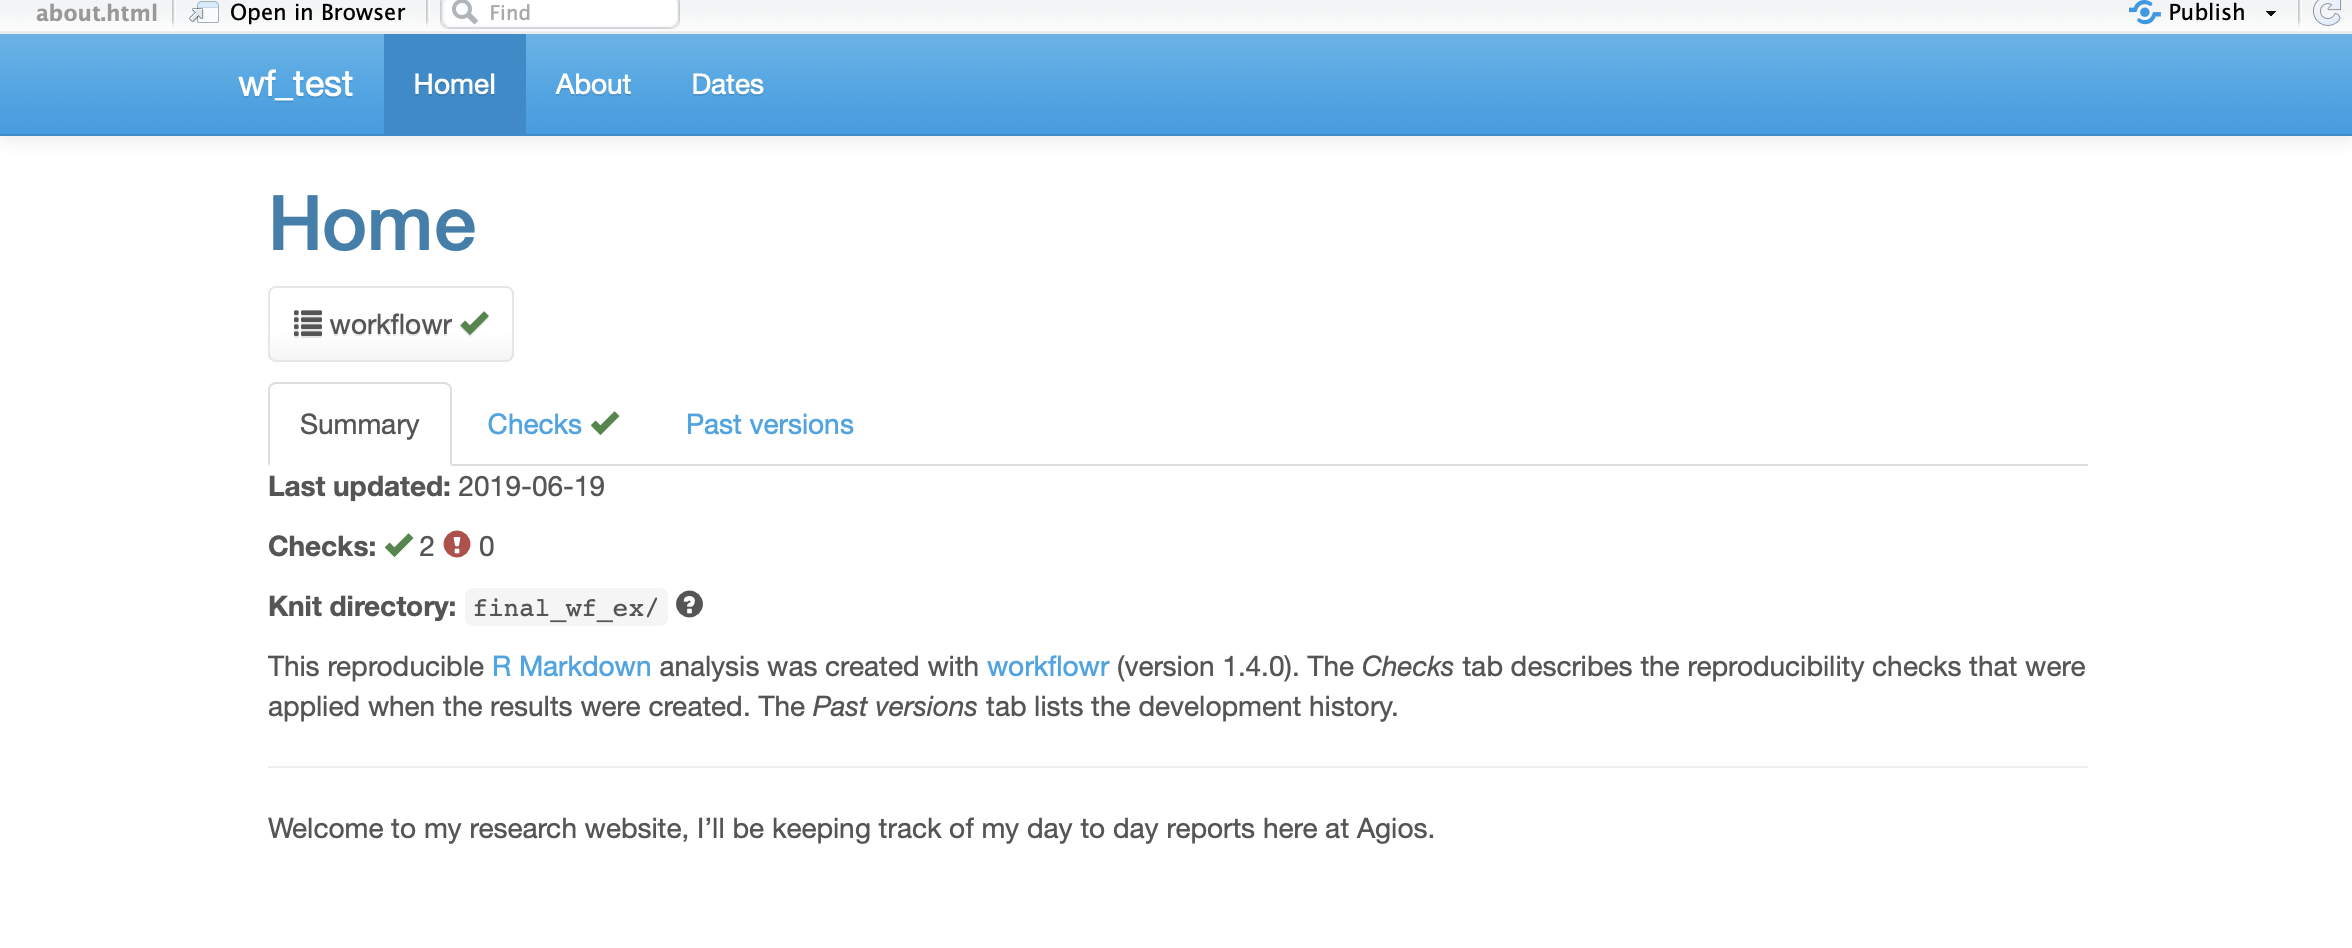
\includegraphics[width=0.9\linewidth]{images/Workflow_Photos/sample_wf} \end{center}

\hypertarget{view-project}{%
\subsubsection{View Project}\label{view-project}}

At any time you can view the current site on your local machine by typing in the \texttt{Console} tab:

\begin{Shaded}
\begin{Highlighting}[]
\KeywordTok{wflow_view}\NormalTok{()}
\end{Highlighting}
\end{Shaded}

\hypertarget{publish-website}{%
\subsubsection{Publish Website}\label{publish-website}}

Currently our project is simply an HTML file stored on our laptop, publishing the website will make it available online.

In the \texttt{Console} tab:

\begin{Shaded}
\begin{Highlighting}[]
\KeywordTok{wflow_status}\NormalTok{()}
\end{Highlighting}
\end{Shaded}

This allows you to view which files are published or unpublished currently.

Now we want to publish our page the command to do so takes three parts

\begin{enumerate}
\def\labelenumi{\arabic{enumi}.}
\tightlist
\item
  c - Commit
\item
  (``analysis/index.Rmd'', ``analysis/about.Rmd'', ``analysis/license.Rmd''), - A character vector of the Rmd files you want published

  \begin{itemize}
  \tightlist
  \item
    It may be eaiser to place ("*.Rmd") here to use all the files
  \end{itemize}
\item
  ``Publish the initial files'' - A commit message to be posted
\end{enumerate}

Overall, \texttt{wflow\_publish} is a quick and error-free way for us to commit and push all of our Rmd files to GitLab at once.

In the \texttt{Console} tab:

\begin{Shaded}
\begin{Highlighting}[]
\KeywordTok{wflow_publish}\NormalTok{(}\KeywordTok{c}\NormalTok{(}\StringTok{"analysis/index.Rmd"}\NormalTok{, }\StringTok{"analysis/about.Rmd"}\NormalTok{, }\StringTok{"analysis/license.Rmd"}\NormalTok{), }\StringTok{"Publish the initial files for PROJECT_NAME"}\NormalTok{)}
\end{Highlighting}
\end{Shaded}

\hypertarget{connecting-to-gitlab-1}{%
\subsection{Connecting to GitLab}\label{connecting-to-gitlab-1}}

\hypertarget{creating-a-remote-repository-on-gitlab}{%
\subsubsection{Creating a remote repository on GitLab}\label{creating-a-remote-repository-on-gitlab}}

\begin{enumerate}
\def\labelenumi{\arabic{enumi}.}
\tightlist
\item
  Login to GitLab and click \texttt{New\ Project}
\item
  The project name in GitLab should the same name as the project in RStudio, we called ours PROJECT\_NAME
\item
  Make sure to save it as Internal so everyone in Agios can see it
\end{enumerate}

\hypertarget{connect-rstudio-and-gitlab}{%
\subsubsection{Connect RStudio and GitLab}\label{connect-rstudio-and-gitlab}}

\begin{enumerate}
\def\labelenumi{\arabic{enumi}.}
\tightlist
\item
  Go to RStudio, in \texttt{Console} tab:
\end{enumerate}

\begin{Shaded}
\begin{Highlighting}[]
 \KeywordTok{wflow_use_gitlab}\NormalTok{(}\DataTypeTok{username =} \StringTok{"first.last"}\NormalTok{, }\DataTypeTok{repository =} \StringTok{"PROJECT_NAME"}\NormalTok{, }\DataTypeTok{domain =} \StringTok{"ceres.agios.com"}\NormalTok{)}
\end{Highlighting}
\end{Shaded}

\begin{enumerate}
\def\labelenumi{\arabic{enumi}.}
\setcounter{enumi}{1}
\tightlist
\item
  Go back to GitLab and and scroll down to the \texttt{push\ an\ existing\ Git\ repository} option

  \begin{itemize}
  \tightlist
  \item
    Then, copy every thing in the box besides the \texttt{cd} line
  \end{itemize}
\end{enumerate}

\begin{Shaded}
\begin{Highlighting}[]
\NormalTok{git remote rename origin old}\OperatorTok{-}\NormalTok{origin}
\NormalTok{git remote add origin git}\OperatorTok{@}\NormalTok{ceres.agios.com}\OperatorTok{:}\NormalTok{Caitlin.Guccione}\OperatorTok{/}\NormalTok{test}\OperatorTok{-}\NormalTok{.git}
\NormalTok{git push }\OperatorTok{-}\NormalTok{u origin }\OperatorTok{--}\NormalTok{all}
\NormalTok{git push }\OperatorTok{-}\NormalTok{u origin }\OperatorTok{--}\NormalTok{tags}
\end{Highlighting}
\end{Shaded}

\begin{enumerate}
\def\labelenumi{\arabic{enumi}.}
\setcounter{enumi}{2}
\tightlist
\item
  Go back into RStudio and in the \texttt{Terminal} tab

  \begin{itemize}
  \tightlist
  \item
    Make sure you are in the PROJECT\_NAME repo
  \item
    Paste the above commands
  \end{itemize}
\item
  Return to GitLab to ensure your entire project exists there
\end{enumerate}

\begin{figure}

{\centering 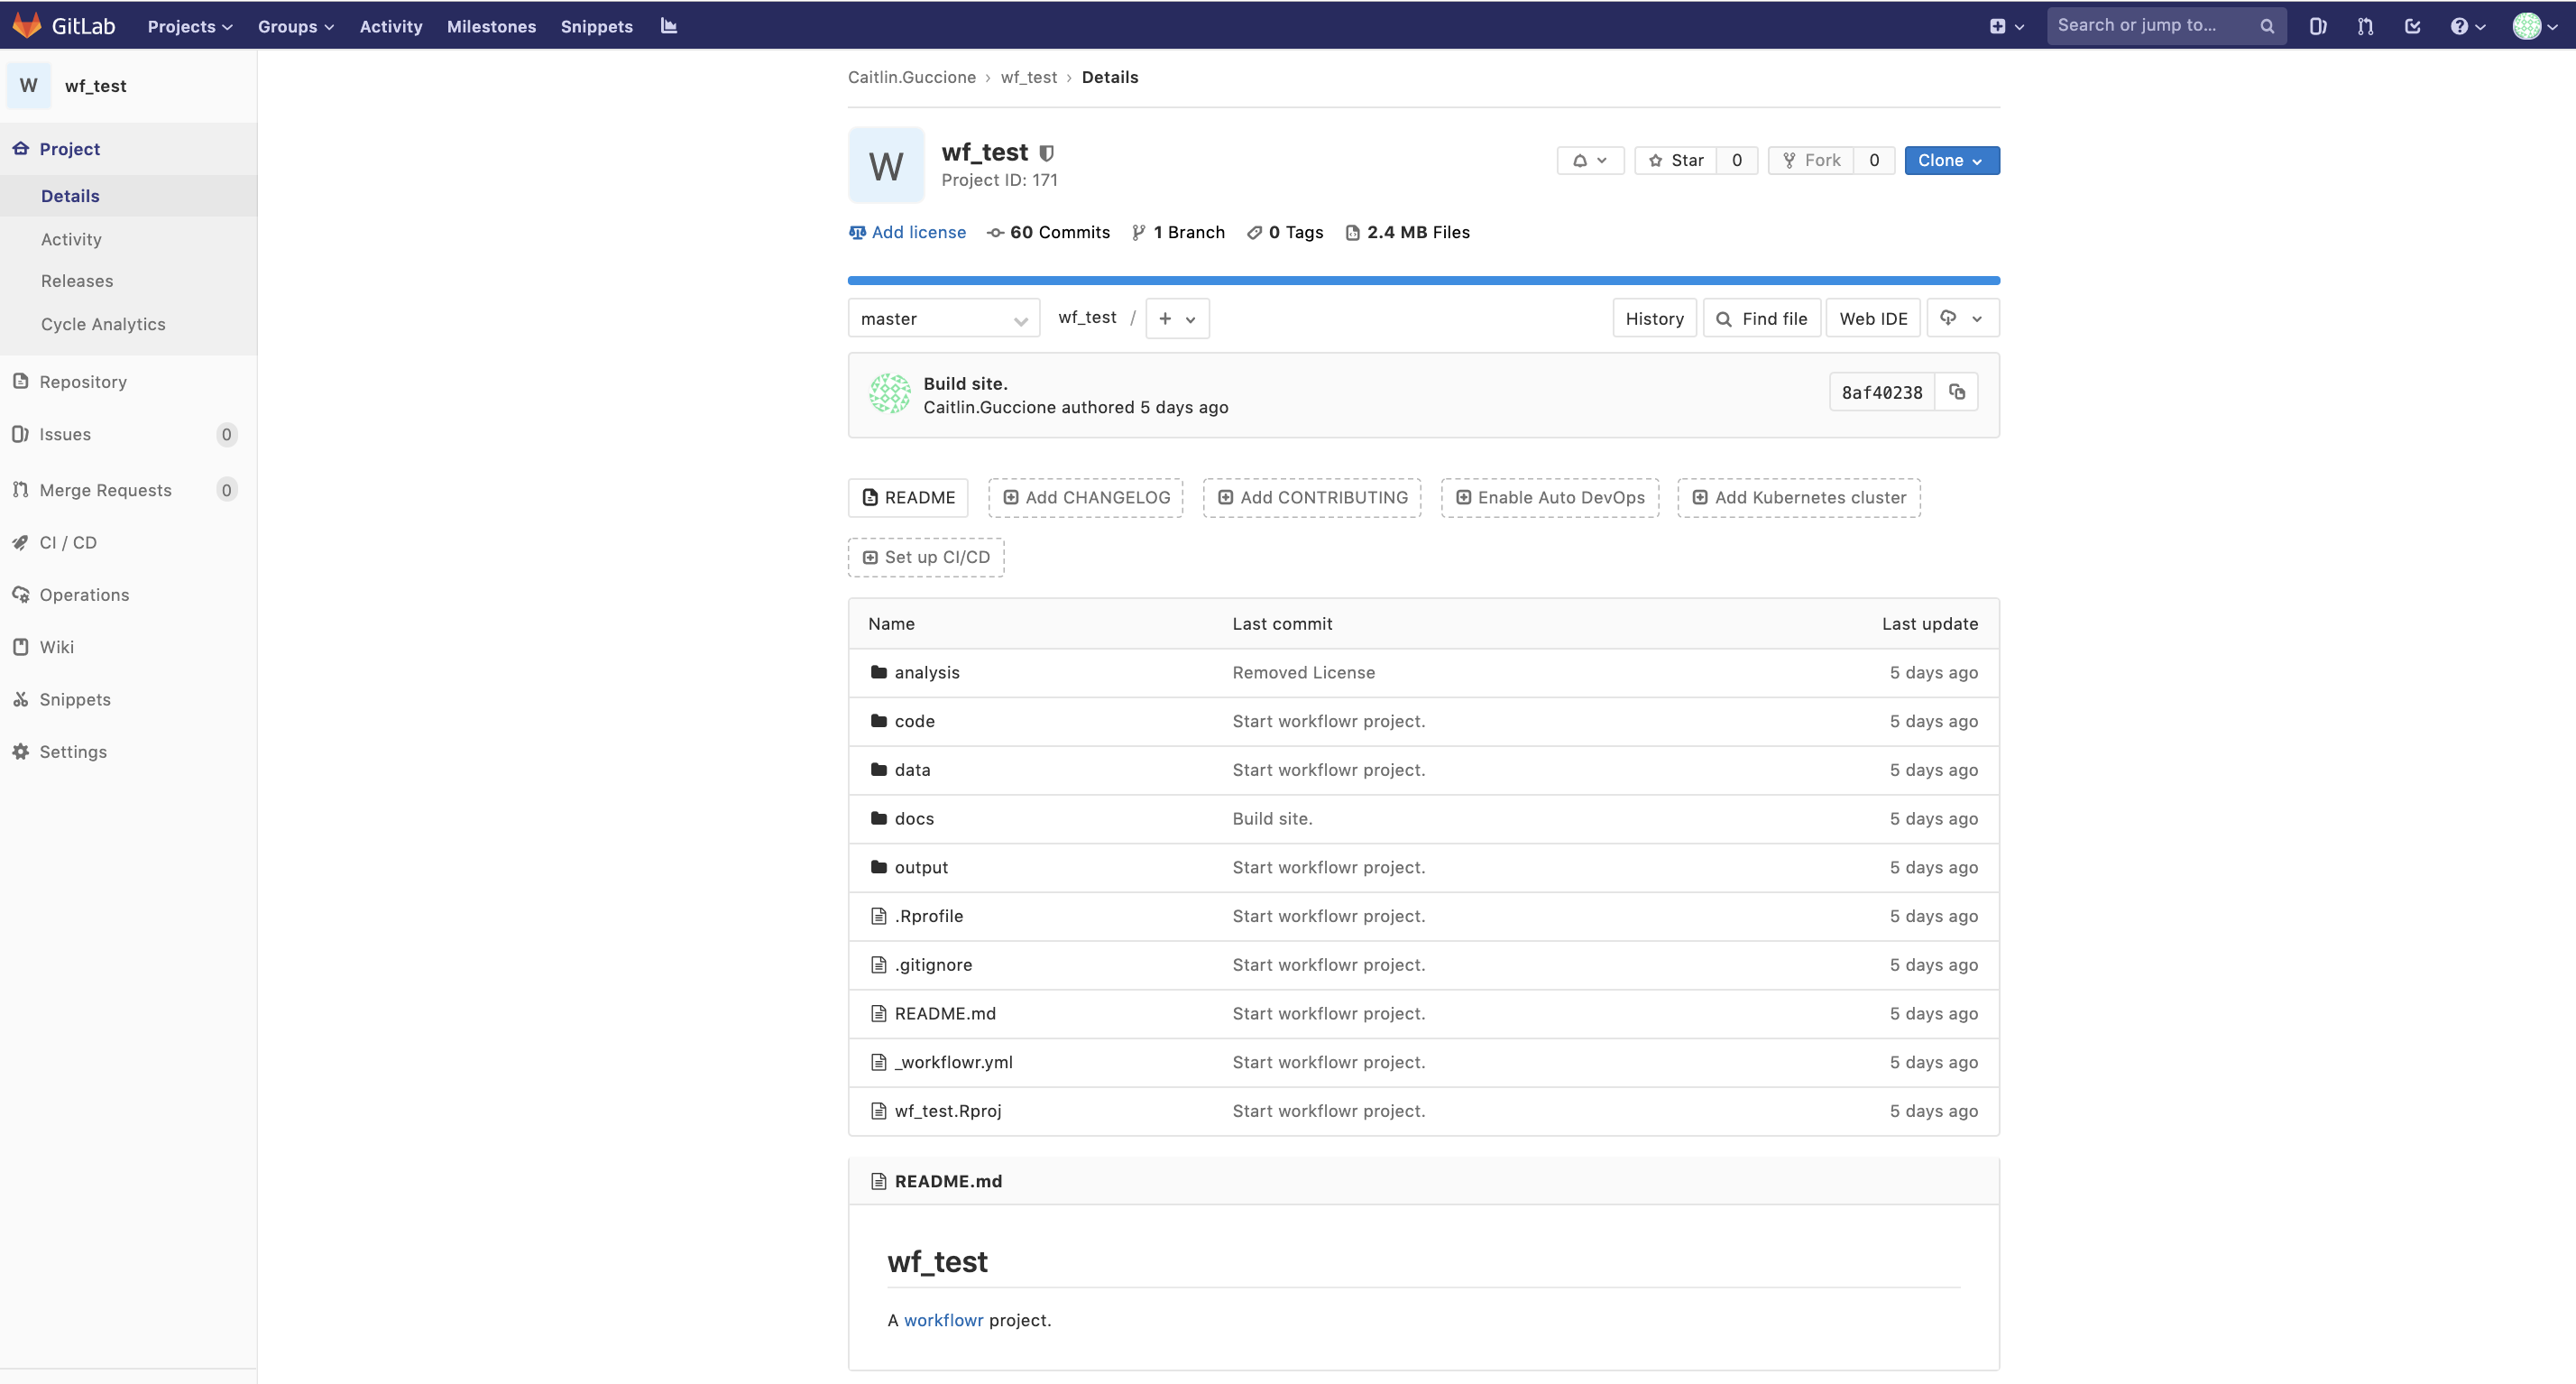
\includegraphics[width=1\linewidth]{images/Workflow_Photos/screen_shot} 

}

\caption{Example GitLab and Workflowr Connection}\label{fig:a3}
\end{figure}

\hypertarget{adding-new-files}{%
\subsection{Adding New Files}\label{adding-new-files}}

\hypertarget{creating-new-files}{%
\subsubsection{Creating New Files}\label{creating-new-files}}

Make sure you are inside the PROJECT\_NAME project inside RStudio

In \texttt{Console} tab type:

\begin{Shaded}
\begin{Highlighting}[]
\KeywordTok{wflow_open}\NormalTok{(}\StringTok{"analysis/NEW_FILE.Rmd"}\NormalTok{)}
\end{Highlighting}
\end{Shaded}

\begin{itemize}
\tightlist
\item
  This command creates a new Rmd file and then opens it for your convivence.
\end{itemize}

If we now want to see the HTML version of our file then we have two options:

\begin{enumerate}
\def\labelenumi{\arabic{enumi}.}
\tightlist
\item
  In \texttt{Console} tab type:
\end{enumerate}

\begin{Shaded}
\begin{Highlighting}[]
\KeywordTok{wflow_build}\NormalTok{()}
\end{Highlighting}
\end{Shaded}

\begin{itemize}
\tightlist
\item
  You can add specfic files to this command or simply leave it empty
\item
  This produces a small view of your website right on RStudio
\end{itemize}

\begin{enumerate}
\def\labelenumi{\arabic{enumi}.}
\setcounter{enumi}{1}
\tightlist
\item
  Press the `Knit' button in RStudio as shown below:
\end{enumerate}

\begin{center}
\includegraphics[width=0.1\linewidth]{images/Workflow_Photos/knit} \end{center}

\begin{itemize}
\tightlist
\item
  This produces a large web version of your current HTML file
\end{itemize}

These steps will simply change the HTML file local bu tin order to make this public and add it to GitLab we need to update our changes.

\hypertarget{update-your-changes}{%
\subsubsection{Update your Changes}\label{update-your-changes}}

\begin{enumerate}
\def\labelenumi{\arabic{enumi}.}
\tightlist
\item
  Check the status to see what needs to be udated, in the \texttt{Console} tab,
\end{enumerate}

\begin{Shaded}
\begin{Highlighting}[]
\KeywordTok{wflow_status}\NormalTok{()}
\end{Highlighting}
\end{Shaded}

This can also be done by looking at the red checks on the workflowr section of your live page as shown below:

\begin{center}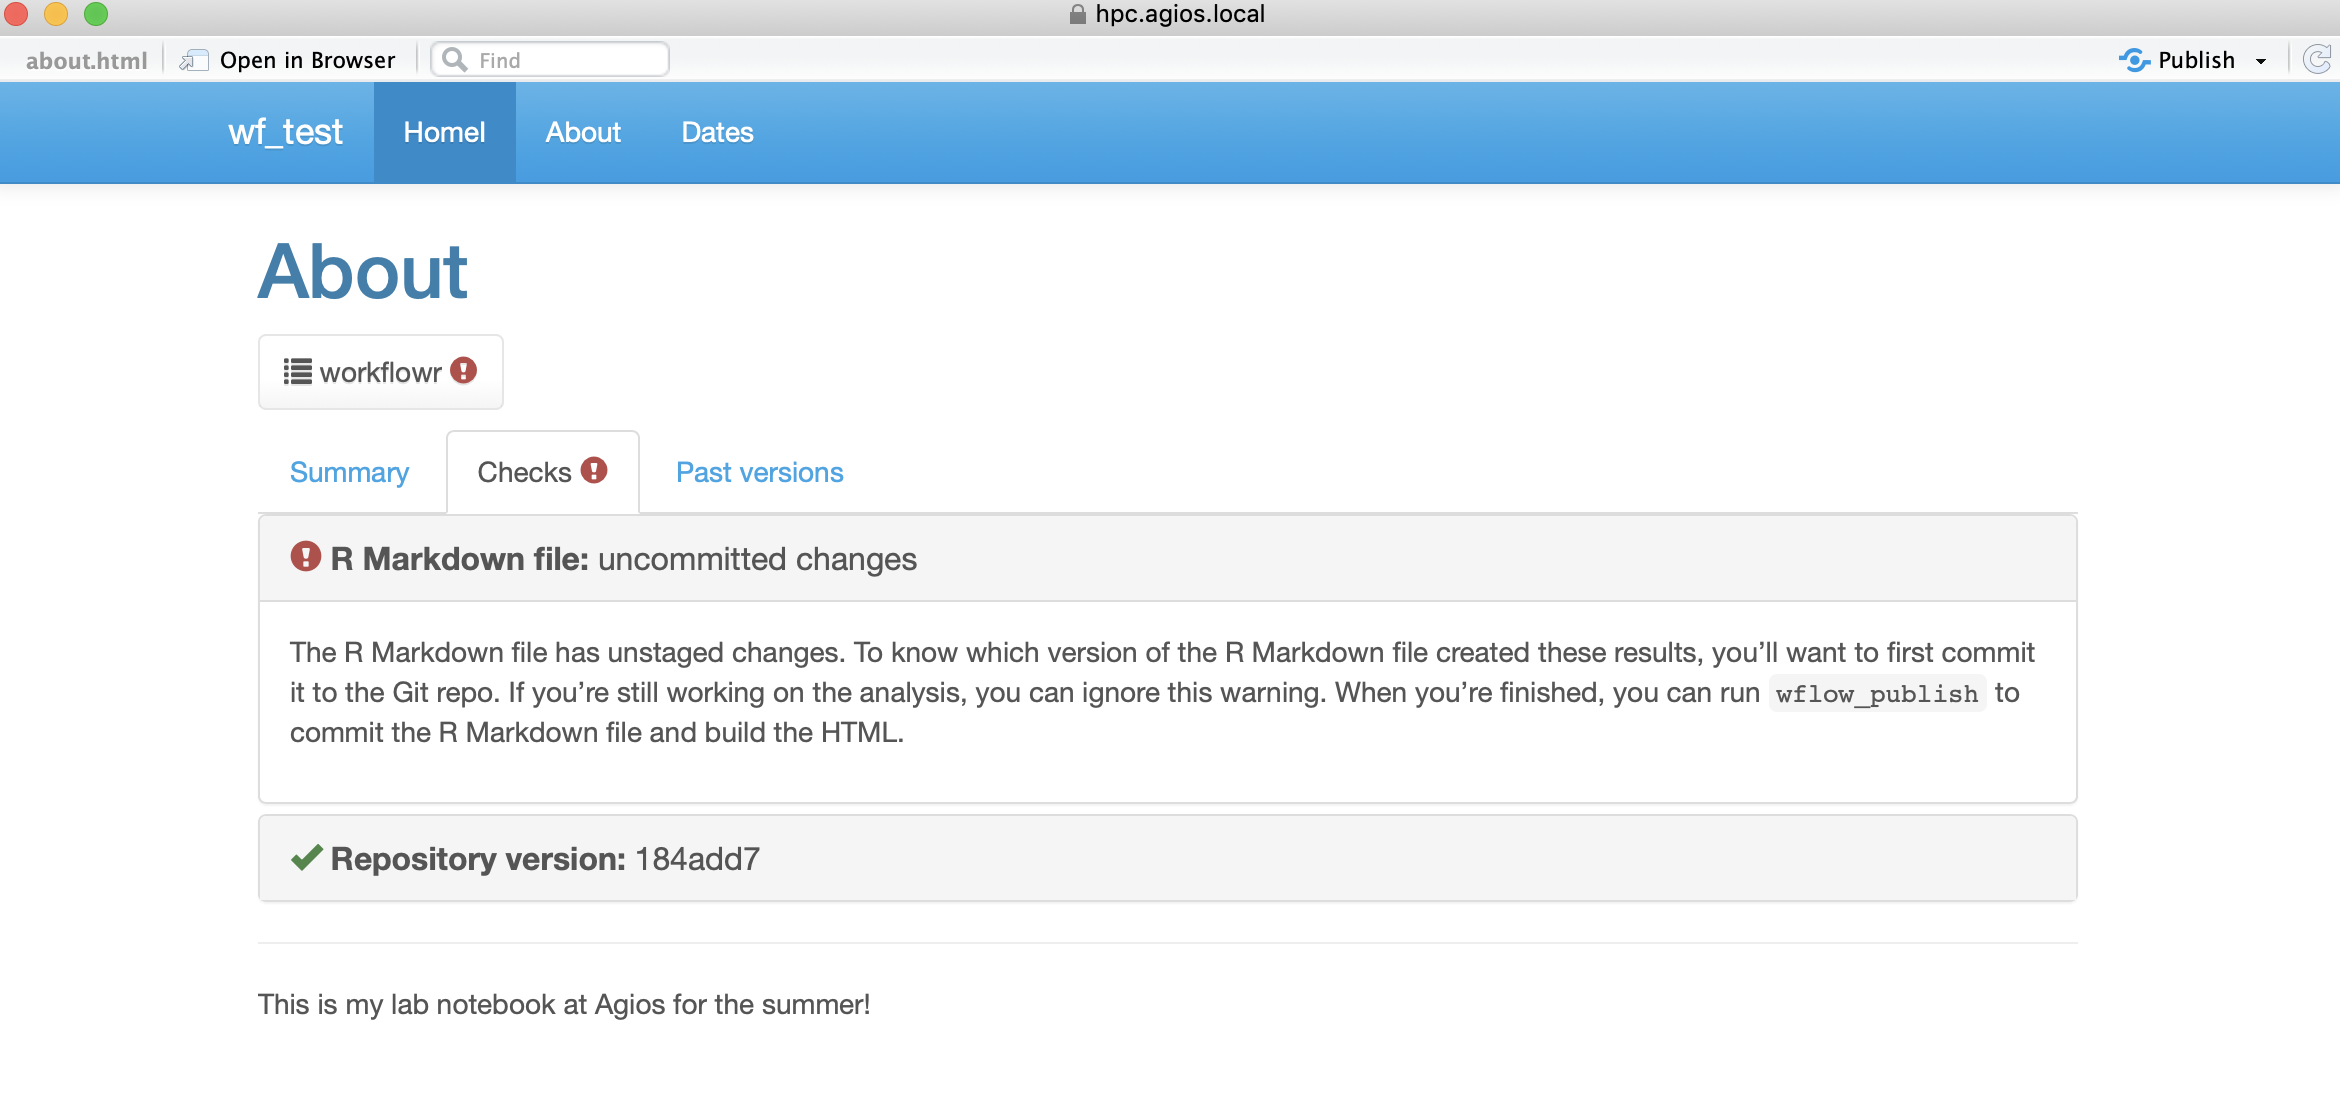
\includegraphics[width=0.9\linewidth]{images/Workflow_Photos/red_checks} \end{center}

\begin{enumerate}
\def\labelenumi{\arabic{enumi}.}
\setcounter{enumi}{1}
\tightlist
\item
  Make the appropriate HTML files public and updated, in the \texttt{Console} tab,
\end{enumerate}

\begin{Shaded}
\begin{Highlighting}[]
\KeywordTok{wflow_publish}\NormalTok{(}\KeywordTok{c}\NormalTok{(}\StringTok{"analysis/index.Rmd"}\NormalTok{, }\StringTok{"analysis/NEW_FILE.Rmd"}\NormalTok{), }\StringTok{"Add my first file"}\NormalTok{)}
\end{Highlighting}
\end{Shaded}

\begin{itemize}
\tightlist
\item
  This is the same format found on the \texttt{Publish\ Website} tab of this page and so you can customize it in the same way
\end{itemize}

There is one exception to this and it's when you want to make updates to the \texttt{\_site.yml} file found in the \texttt{analysis} folder. This file controls the style on the top of every page of your website. In this case you want to update all HTML files even though their Rmd files aren't changed.

In that case, use this,

\begin{Shaded}
\begin{Highlighting}[]
\KeywordTok{wflow_publish}\NormalTok{(}\StringTok{"analysis/_site.yml"}\NormalTok{, }\StringTok{"Change the theme"}\NormalTok{, }\DataTypeTok{republish =} \OtherTok{TRUE}\NormalTok{)}
\end{Highlighting}
\end{Shaded}

\begin{enumerate}
\def\labelenumi{\arabic{enumi}.}
\setcounter{enumi}{2}
\tightlist
\item
  Push the final changes to GitLab
\end{enumerate}

As we did previously in the \texttt{Publish\ Website}, in the \texttt{Terminal} tab,

\begin{Shaded}
\begin{Highlighting}[]
\NormalTok{git push}
\end{Highlighting}
\end{Shaded}

\hypertarget{adding-workflowr-to-new-file}{%
\subsubsection{Adding Workflowr to New File}\label{adding-workflowr-to-new-file}}

If you want the normal workflowr setup which is found on all the other pages, then replace the --- part of the file with the following code:

\begin{verbatim}
            ---
            title: "Home"
            site: workflowr::wflow_site
            output:
              workflowr::wflow_html:
                toc: false
            editor_options:
              chunk_output_type: console
      ---
\end{verbatim}

\hypertarget{styling-the-webpage}{%
\subsection{Styling the Webpage}\label{styling-the-webpage}}

\hypertarget{helpful-links}{%
\subsubsection{Helpful Links}\label{helpful-links}}

If you already have an idea of what you would like to change, below are a few very helpful resources filled with information:

\begin{itemize}
\tightlist
\item
  This resource is a great place to start because it has all basics of Rmd syntax and I used it as a cheat sheet along the way.

  \begin{itemize}
  \tightlist
  \item
    \href{https://rmarkdown.rstudio.com/authoring_basics.html}{Rmd Cheat Sheet}
  \end{itemize}
\item
  This is an entire book all about Rmd and how to use it. I found it rather lengthy but very helpful.

  \begin{itemize}
  \tightlist
  \item
    \href{https://bookdown.org/yihui/rmarkdown/html-document.html\#appearance_and_style}{Rmd Thorough Guide}
  \end{itemize}
\item
  If something isn't quite working right you may have run into a workflowr issue in which cause thier FAQ's page is helpful.

  \begin{itemize}
  \tightlist
  \item
    \href{https://jdblischak.github.io/workflowr/articles/wflow-05-faq.html}{Workflor FAQ's}
  \end{itemize}
\end{itemize}

\hypertarget{changing-the-theme}{%
\subsubsection{Changing the Theme}\label{changing-the-theme}}

Changing the theme modifies the overall apparane of the webpage is a quick and easy way to spice up the page.

\begin{enumerate}
\def\labelenumi{\arabic{enumi}.}
\tightlist
\item
  Go into your \texttt{analysis/\_site.yml} file
\item
  Underneath \texttt{ouput} add \texttt{theme\ =\ cerulean} as shown below:

  \begin{itemize}
  \tightlist
  \item
    The cerulean theme matches Agios colors
  \end{itemize}
\end{enumerate}

\begin{Shaded}
\begin{Highlighting}[]
\NormalTok{output}\OperatorTok{:}
\StringTok{    }\NormalTok{theme}\OperatorTok{:}\StringTok{ }\NormalTok{cerulean}
\end{Highlighting}
\end{Shaded}

\begin{enumerate}
\def\labelenumi{\arabic{enumi}.}
\setcounter{enumi}{2}
\tightlist
\item
  Choose your theme

  \begin{itemize}
  \tightlist
  \item
    The following themes are avalible : ``default'', ``cerulean'', ``journal'', ``flatly'', ``darkly'', ``readable'', ``spacelab'', ``united'', ``cosmo'', ``lumen'', ``paper'', ``sandstone'', ``simplex'', ``yeti''
  \item
    You can view how they look here: \href{https://bootswatch.com/}{Themes}
  \end{itemize}
\item
  Preview your theme using,
\end{enumerate}

\begin{Shaded}
\begin{Highlighting}[]
\KeywordTok{wflow_build}\NormalTok{()}
\end{Highlighting}
\end{Shaded}

\begin{enumerate}
\def\labelenumi{\arabic{enumi}.}
\setcounter{enumi}{4}
\tightlist
\item
  Update your website by running,

  \begin{itemize}
  \tightlist
  \item
    This will rebuild every HTML file even if thier corresponding Rmd file hasn't been updated
  \end{itemize}
\end{enumerate}

\begin{Shaded}
\begin{Highlighting}[]
\KeywordTok{wflow_publish}\NormalTok{(}\StringTok{"analysis/_site.yml"}\NormalTok{, }\StringTok{"Change the theme"}\NormalTok{, }\DataTypeTok{republish =} \OtherTok{TRUE}\NormalTok{)}
\end{Highlighting}
\end{Shaded}

The following website will also walk you through changing the theme: \href{https://jdblischak.github.io/workflowr/articles/wflow-02-customization.html\#changing-the-theme}{Themes Overview}

\hypertarget{adding-photos}{%
\subsubsection{Adding Photos}\label{adding-photos}}

Although this may seem like a simple taks, it is a bit challenging since we are using Workflowr

\begin{enumerate}
\def\labelenumi{\arabic{enumi}.}
\tightlist
\item
  Create a \texttt{photos} folder inside the \texttt{docs} folder and add your photo there:
\end{enumerate}

\begin{Shaded}
\begin{Highlighting}[]
\KeywordTok{dir.create}\NormalTok{(}\StringTok{"docs/photos"}\NormalTok{)}
\end{Highlighting}
\end{Shaded}

\begin{enumerate}
\def\labelenumi{\arabic{enumi}.}
\setcounter{enumi}{1}
\tightlist
\item
  Include the following command wherever you want your graphic to apper:
\end{enumerate}

\begin{flushleft}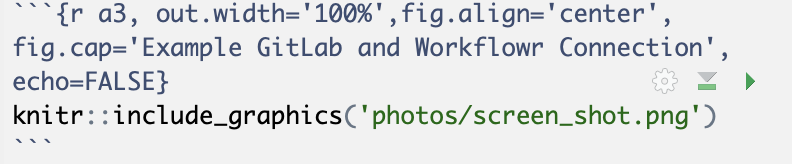
\includegraphics[width=0.5\linewidth]{images/Workflow_Photos/photoExample} \end{flushleft}

\begin{enumerate}
\def\labelenumi{\arabic{enumi}.}
\setcounter{enumi}{2}
\tightlist
\item
  View the images on the webpage
\end{enumerate}

\begin{Shaded}
\begin{Highlighting}[]
\KeywordTok{wflow_build}\NormalTok{()}
\end{Highlighting}
\end{Shaded}

\begin{enumerate}
\def\labelenumi{\arabic{enumi}.}
\setcounter{enumi}{3}
\tightlist
\item
  Add to GitLab

  \begin{itemize}
  \tightlist
  \item
    We need to push the acutal photo to GitLab using \texttt{wflow\_git\_commit} and then we can use \texttt{wflow\_publish} to automatically push the rest of the files to GitLab
  \end{itemize}
\end{enumerate}

\begin{Shaded}
\begin{Highlighting}[]
\KeywordTok{wflow_git_commit}\NormalTok{(}\StringTok{"docs/assets/external.png"}\NormalTok{, }\StringTok{"Add external image of ..."}\NormalTok{)}
\KeywordTok{wflow_publish}\NormalTok{()}
\end{Highlighting}
\end{Shaded}

\hypertarget{set-up-workflow-and-executing}{%
\section{Set Up Workflow and Executing}\label{set-up-workflow-and-executing}}

\hypertarget{create-a-folder-for-your-newproject}{%
\subsection{\texorpdfstring{Create a folder for your \emph{newproject}}{Create a folder for your newproject}}\label{create-a-folder-for-your-newproject}}

Come up with a project stucture you like and stick with it.

\hypertarget{copy-from-a-previously-created-template-folder}{%
\subsubsection{Copy from a previously created template folder}\label{copy-from-a-previously-created-template-folder}}

Use \texttt{cp\ -r\ project\_template\ newproject}, where \texttt{project\_template} has structure:

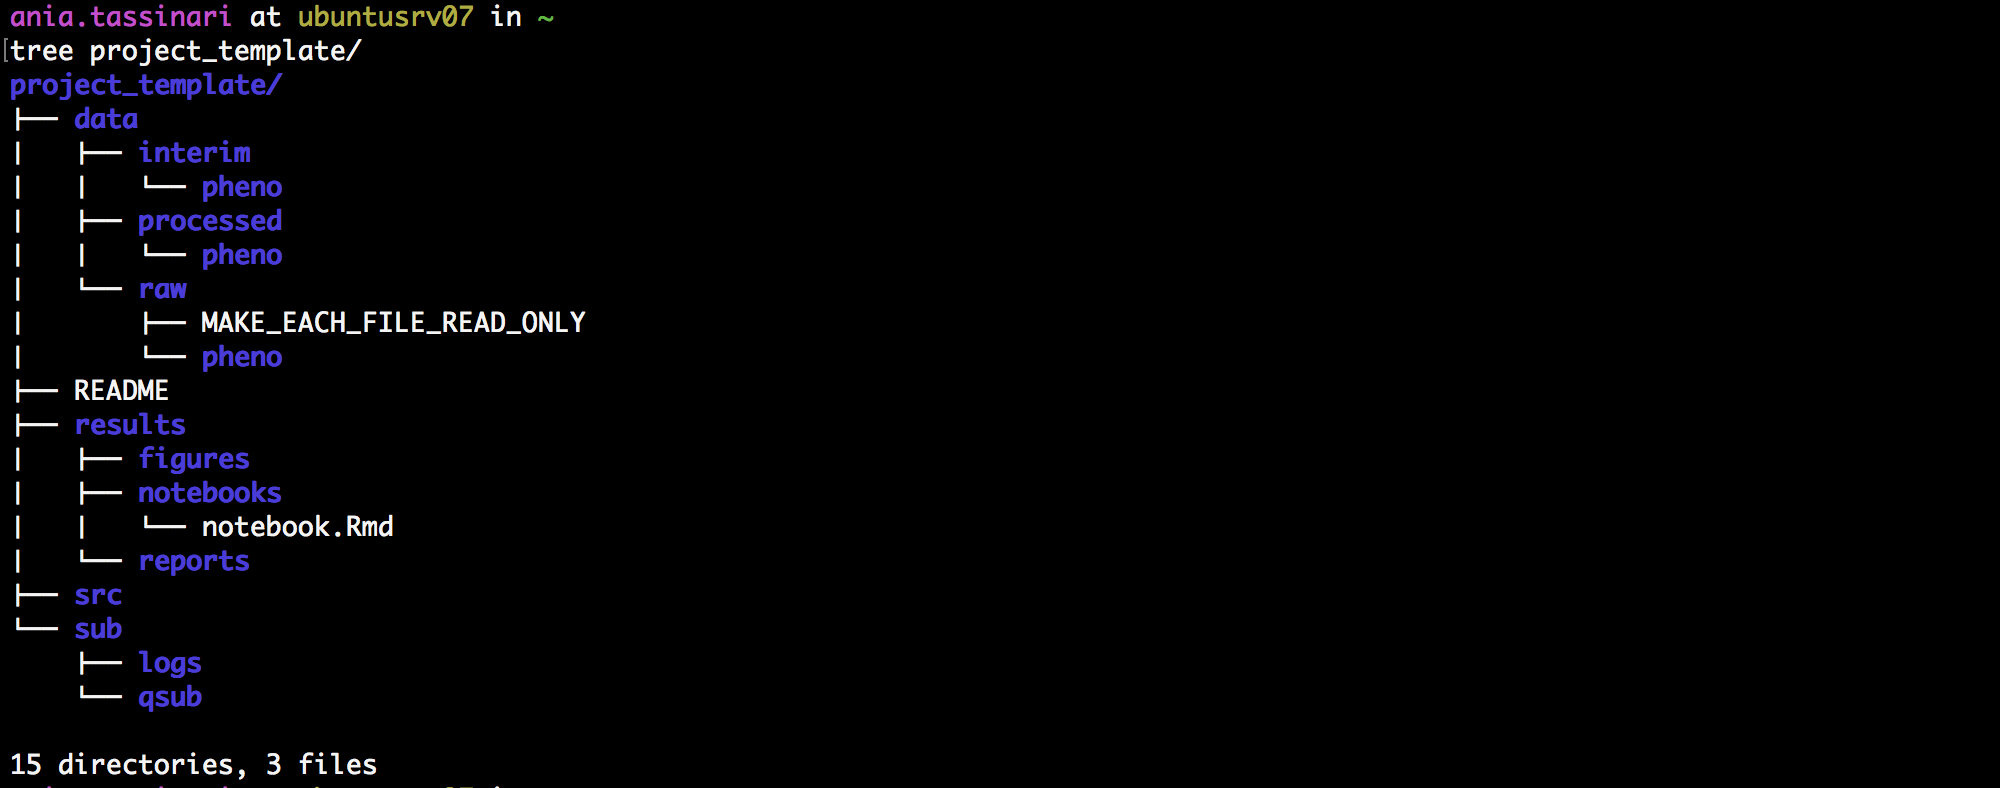
\includegraphics[width=27.78in]{images/projectstructure}

\hypertarget{use-a-bash-script}{%
\subsubsection{\texorpdfstring{Use a \texttt{bash} script}{Use a bash script}}\label{use-a-bash-script}}

Call \texttt{./setup\_project.sh\ newproject}, where \texttt{setup\_project.sh} is:

Don't forget!
- Fill project README
- Adapt structure to project needs
- Exclude data and other large files from git using \texttt{.gitignore} (see next section)
- Make files in \texttt{data/raw} read-only with \texttt{chmod\ -w}

Project organization ideas:
\url{http://projecttemplate.net/getting_started.html}
Packaging data analytical work reproducibly using R (and friends)
R workflow fun
Cookiecutter Data Science

\hypertarget{set-up-a-repository-for-your-code-on-agios-secure-gitlab}{%
\subsection{Set up a repository for your code on Agios' secure GitLab}\label{set-up-a-repository-for-your-code-on-agios-secure-gitlab}}

Create a new project at http://ceres.agios.com (Mark P. can help)

\hypertarget{set-up-a-repository-for-your-code-locally-and-link-to-gitlab}{%
\subsection{Set up a repository for your code locally and link to GitLab}\label{set-up-a-repository-for-your-code-locally-and-link-to-gitlab}}

In your \emph{newproject} folder on command line execute (modify user name):

\hypertarget{set-up-an-r-project-in-rstudio}{%
\subsection{Set up an R project in RStudio}\label{set-up-an-r-project-in-rstudio}}

Choose Existing Directory (\emph{newproject})

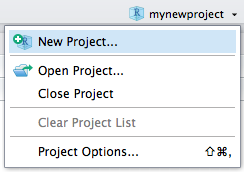
\includegraphics[width=3.39in]{images/newproject0}
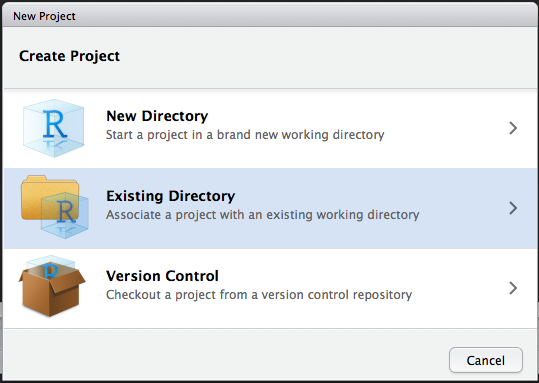
\includegraphics[width=7.49in]{images/newproject}

\hypertarget{analysis-in-r-and-rstudio}{%
\subsection{Analysis in R and RStudio}\label{analysis-in-r-and-rstudio}}

\textbf{Data:}

\begin{itemize}
\tightlist
\item
  Raw data:

  \begin{itemize}
  \tightlist
  \item
    If accessed from the web, include url, description, and date accessed in README
  \end{itemize}
\item
  Processed:

  \begin{itemize}
  \tightlist
  \item
    Processed data should be named so it is easy to see which script generated the data

    \begin{itemize}
    \tightlist
    \item
      Can add file descriptions to \texttt{filename.README} and place processing script in the same directory as data (works well for preprocessing steps, like alignments, etc)
    \end{itemize}
  \item
    Processed data should be tidy
  \end{itemize}
\end{itemize}

\textbf{Code:}

\begin{itemize}
\tightlist
\item
  Place (almost) all intermediate scripts in \texttt{newproject/src/}
\item
  Any chunks of code frequently reused in the analysis should be converted into functions, saved in \texttt{newproject/src/functions.R}, and sourced in scripts, notebooks and reports.\\
\item
  Use Google's R Style Guide or The tidyverse styleguide to format your code and make it easier to read (if need be run code through formatR)
\end{itemize}

\textbf{Figures:}

\begin{itemize}
\tightlist
\item
  Exploratory:

  \begin{itemize}
  \tightlist
  \item
    Don't have to be pretty
  \item
    Can be embedded in report / notebook
  \end{itemize}
\item
  Final:

  \begin{itemize}
  \tightlist
  \item
    Should be polished and saved in \texttt{newproject/results/figures/}
  \end{itemize}
\end{itemize}

\textbf{Scripts:}

\begin{itemize}
\tightlist
\item
  Raw:

  \begin{itemize}
  \tightlist
  \item
    May be less commented (but comments help you!)
  \item
    May be multiple versions
  \item
    May include analyses that are later discarded
  \end{itemize}
\item
  Final:

  \begin{itemize}
  \tightlist
  \item
    Clearly commented
  \item
    Small comments liberally - what, when, why, how
  \item
    Bigger commented blocks for whole sections
  \item
    Include processing details
  \item
    Only analyses that appear in the final write-up
  \end{itemize}
\end{itemize}

\textbf{Notebooks and reports:}

\begin{itemize}
\item
  R markdown files can be used to generate reproducible reports
\item
  Text and R code are integrated
\item
  Notebooks:

  \begin{itemize}
  \tightlist
  \item
    intermediate
  \item
    may use one per day or one per subanalysis
  \item
    documents all atempts
  \end{itemize}
\item
  Reports:

  \begin{itemize}
  \tightlist
  \item
    final methods and results only
  \item
    good for sharing
  \end{itemize}
\end{itemize}

Adapted from: Reproducible Research at Coursera

\hypertarget{version-control-in-git-and-gitlab}{%
\subsection{Version control in git and GitLab}\label{version-control-in-git-and-gitlab}}

Adopt a branching workflow appropriate for the project and team size, and stick to it.

\url{gitforsmallteams}

Reprinted from: Git workflow for small teams. Link currently is password protected.

\textbf{\texttt{git} and \texttt{git-workflow} resources:}
Learn git
Git branching model
GitFlow

\hypertarget{keeping-track-of-enviroment}{%
\subsection{Keeping track of enviroment}\label{keeping-track-of-enviroment}}

Use \texttt{devtools::session\_info()}

or \texttt{sessionInfo()}

or \texttt{docker} with \texttt{rrtools}

\hypertarget{toolbox}{%
\chapter{Toolbox}\label{toolbox}}

\hypertarget{command-line-tools}{%
\section{Command Line Tools}\label{command-line-tools}}

\hypertarget{bioinformatics}{%
\subsection{Bioinformatics}\label{bioinformatics}}

\hypertarget{get-average-read-length-from-a-.bam-file}{%
\subsubsection{\texorpdfstring{Get average read length from a \texttt{.bam} file}{Get average read length from a .bam file}}\label{get-average-read-length-from-a-.bam-file}}

\begin{Shaded}
\begin{Highlighting}[]
\ExtensionTok{samtools}\NormalTok{ view sorted.bam }\KeywordTok{|} \FunctionTok{head}\NormalTok{ -n 1000000 }\KeywordTok{|} \FunctionTok{cut}\NormalTok{ -f 10 }\KeywordTok{|} \FunctionTok{perl}\NormalTok{ -ne }\StringTok{'chomp;print length($_) . "\textbackslash{}n"'} \KeywordTok{|} \FunctionTok{sort} \KeywordTok{|} \FunctionTok{uniq}\NormalTok{ -c}
\end{Highlighting}
\end{Shaded}

\hypertarget{docker}{%
\subsection{Docker}\label{docker}}

\hypertarget{basic-commands}{%
\subsubsection{Basic commands}\label{basic-commands}}

Here are a few helpful commands for working with \texttt{docker} images

\begin{Shaded}
\begin{Highlighting}[]
\ExtensionTok{docker}\NormalTok{ ps -a               # Lists containers (and tells you which images they are spun from)}
\ExtensionTok{docker}\NormalTok{ images              # Lists images  }
\ExtensionTok{docker}\NormalTok{ rm }\OperatorTok{<}\NormalTok{container_id}\OperatorTok{>}\NormalTok{   # Removes a container}

\ExtensionTok{docker}\NormalTok{ rmi }\OperatorTok{<}\NormalTok{image_id}\OperatorTok{>}\NormalTok{      # Removes an image }
                           \CommentTok{# Will fail if there is a running instance of that image i.e. container}

\ExtensionTok{docker}\NormalTok{ rmi -f }\OperatorTok{<}\NormalTok{image_id}\OperatorTok{>}\NormalTok{   # Forces removal of image even if it is referenced in multiple repositories, }
                           \CommentTok{# i.e. same image id given multiple names/tags }
                           \CommentTok{# Will still fail if there is a docker container referencing image}
\end{Highlighting}
\end{Shaded}

\hypertarget{pruning}{%
\subsubsection{Pruning}\label{pruning}}

\begin{Shaded}
\begin{Highlighting}[]
\CommentTok{# remove dangling images }
\ExtensionTok{docker}\NormalTok{ rmi }\VariableTok{$(}\ExtensionTok{docker}\NormalTok{ images --filter “dangling=true” -q --no-trunc}\VariableTok{)}

\CommentTok{# find other untagged images (with possible children) (<none>:<none>)}
\ExtensionTok{docker}\NormalTok{ images -a }\KeywordTok{|} \FunctionTok{grep} \StringTok{"none"} \KeywordTok{|} \FunctionTok{awk} \StringTok{'\{print $3\}'}

\CommentTok{# try removing them}
\ExtensionTok{docker}\NormalTok{ rmi }\VariableTok{$(}\ExtensionTok{docker}\NormalTok{ images -a }\KeywordTok{|} \FunctionTok{grep} \StringTok{"none"} \KeywordTok{|} \FunctionTok{awk} \StringTok{'\{print $3\}'}\VariableTok{)}

\CommentTok{# if any left because of clingy children, get __parent.ID__ (ID of untagged image) and then:}
\CommentTok{# example: docker inspect --format='\{\{.Id\}\} \{\{.Parent\}\}' $(docker images --filter since=14a1e7116365 -q)}
\ExtensionTok{docker}\NormalTok{ inspect --format=}\StringTok{'\{\{.Id\}\} \{\{.Parent\}\}'} \VariableTok{$(}\ExtensionTok{docker}\NormalTok{ images --filter since=__parent.id__ -q}\VariableTok{)}

\CommentTok{# then remove listed __children.id__ one by one}
\CommentTok{# example: docker rmi 382096f13260254f3c472bf63f063b8ecbc2d4cc06fe7a940d6fbd4636ef77b1}
\ExtensionTok{docker}\NormalTok{ rmi __child.id__}
\end{Highlighting}
\end{Shaded}

\hypertarget{file-system}{%
\subsection{File system}\label{file-system}}

\hypertarget{list-top-5-largest-files}{%
\subsubsection{List top 5 largest files}\label{list-top-5-largest-files}}

\begin{Shaded}
\begin{Highlighting}[]
\FunctionTok{du}\NormalTok{ -a /path/to/my/dir/ }\KeywordTok{|} \FunctionTok{sort}\NormalTok{ -n -r }\KeywordTok{|} \FunctionTok{head}\NormalTok{ -n 5}
\end{Highlighting}
\end{Shaded}

Example:

\begin{Shaded}
\begin{Highlighting}[]
\FunctionTok{du}\NormalTok{ -a /bin }\KeywordTok{|} \FunctionTok{sort}\NormalTok{ -n -r }\KeywordTok{|} \FunctionTok{head}\NormalTok{ -n 5}
\end{Highlighting}
\end{Shaded}

\begin{verbatim}
## 17652    /bin
## 2016 /bin/busybox
## 1552 /bin/ksh93
## 1088 /bin/bash
## 816  /bin/zsh
\end{verbatim}

\hypertarget{list-files-in-a-folder-separated-by-delimeter}{%
\subsubsection{List files in a folder separated by delimeter}\label{list-files-in-a-folder-separated-by-delimeter}}

\begin{Shaded}
\begin{Highlighting}[]
\FunctionTok{ls}\NormalTok{ -1 /path/to/my/dir/ }\KeywordTok{|} \ExtensionTok{paste}\NormalTok{ -sd }\StringTok{","}\NormalTok{ -}
\end{Highlighting}
\end{Shaded}

Example:

\begin{Shaded}
\begin{Highlighting}[]
\FunctionTok{ls}\NormalTok{ -1 /bin }\KeywordTok{|} \ExtensionTok{paste}\NormalTok{ -sd }\StringTok{","}\NormalTok{ -}
\end{Highlighting}
\end{Shaded}

\begin{verbatim}
## bash,btrfs,btrfsck,btrfs-debug-tree,btrfs-find-root,btrfs-image,btrfs-map-logical,btrfs-select-super,btrfstune,btrfs-zero-log,bunzip2,busybox,bzcat,bzcmp,bzdiff,bzegrep,bzexe,bzfgrep,bzgrep,bzip2,bzip2recover,bzless,bzmore,cat,chacl,chgrp,chmod,chown,chvt,cp,cpio,dash,date,dd,df,dir,dmesg,dnsdomainname,domainname,dumpkeys,echo,ed,egrep,false,fgconsole,fgrep,findmnt,fsck.btrfs,fuser,fusermount,getfacl,grep,gunzip,gzexe,gzip,hostname,ip,journalctl,kbd_mode,keyctl,kill,kmod,ksh,ksh93,less,lessecho,lessfile,lesskey,lesspipe,ln,loadkeys,login,loginctl,lowntfs-3g,ls,lsblk,lsmod,mkdir,mkfs.btrfs,mknod,mktemp,more,mount,mountpoint,mt,mt-gnu,mv,nano,nc,nc.openbsd,netcat,netstat,networkctl,nisdomainname,ntfs-3g,ntfs-3g.probe,ntfscat,ntfscluster,ntfscmp,ntfsfallocate,ntfsfix,ntfsinfo,ntfsls,ntfsmove,ntfsrecover,ntfssecaudit,ntfstruncate,ntfsusermap,ntfswipe,open,openvt,pidof,ping,ping4,ping6,plymouth,ps,pwd,rbash,readlink,red,rksh,rksh93,rm,rmdir,rnano,run-parts,rzsh,sed,setfacl,setfont,setupcon,sh,sh.distrib,sleep,ss,static-sh,stty,su,sync,systemctl,systemd,systemd-ask-password,systemd-escape,systemd-hwdb,systemd-inhibit,systemd-machine-id-setup,systemd-notify,systemd-sysusers,systemd-tmpfiles,systemd-tty-ask-password-agent,tar,tempfile,touch,true,udevadm,ulockmgr_server,umount,uname,uncompress,unicode_start,vdir,wdctl,which,whiptail,ypdomainname,zcat,zcmp,zdiff,zegrep,zfgrep,zforce,zgrep,zless,zmore,znew,zsh,zsh5
\end{verbatim}

\hypertarget{compare-structure-of-two-directories}{%
\subsubsection{Compare structure of two directories}\label{compare-structure-of-two-directories}}

\begin{Shaded}
\begin{Highlighting}[]
\ExtensionTok{vimdiff} \OperatorTok{<(}\BuiltInTok{cd}\NormalTok{ dir1}\KeywordTok{;} \FunctionTok{find}\NormalTok{ . }\KeywordTok{|} \FunctionTok{sort}\OperatorTok{)} \OperatorTok{<(}\BuiltInTok{cd}\NormalTok{ dir2}\KeywordTok{;} \FunctionTok{find}\NormalTok{ . }\KeywordTok{|} \FunctionTok{sort}\OperatorTok{)}
\end{Highlighting}
\end{Shaded}

Example:

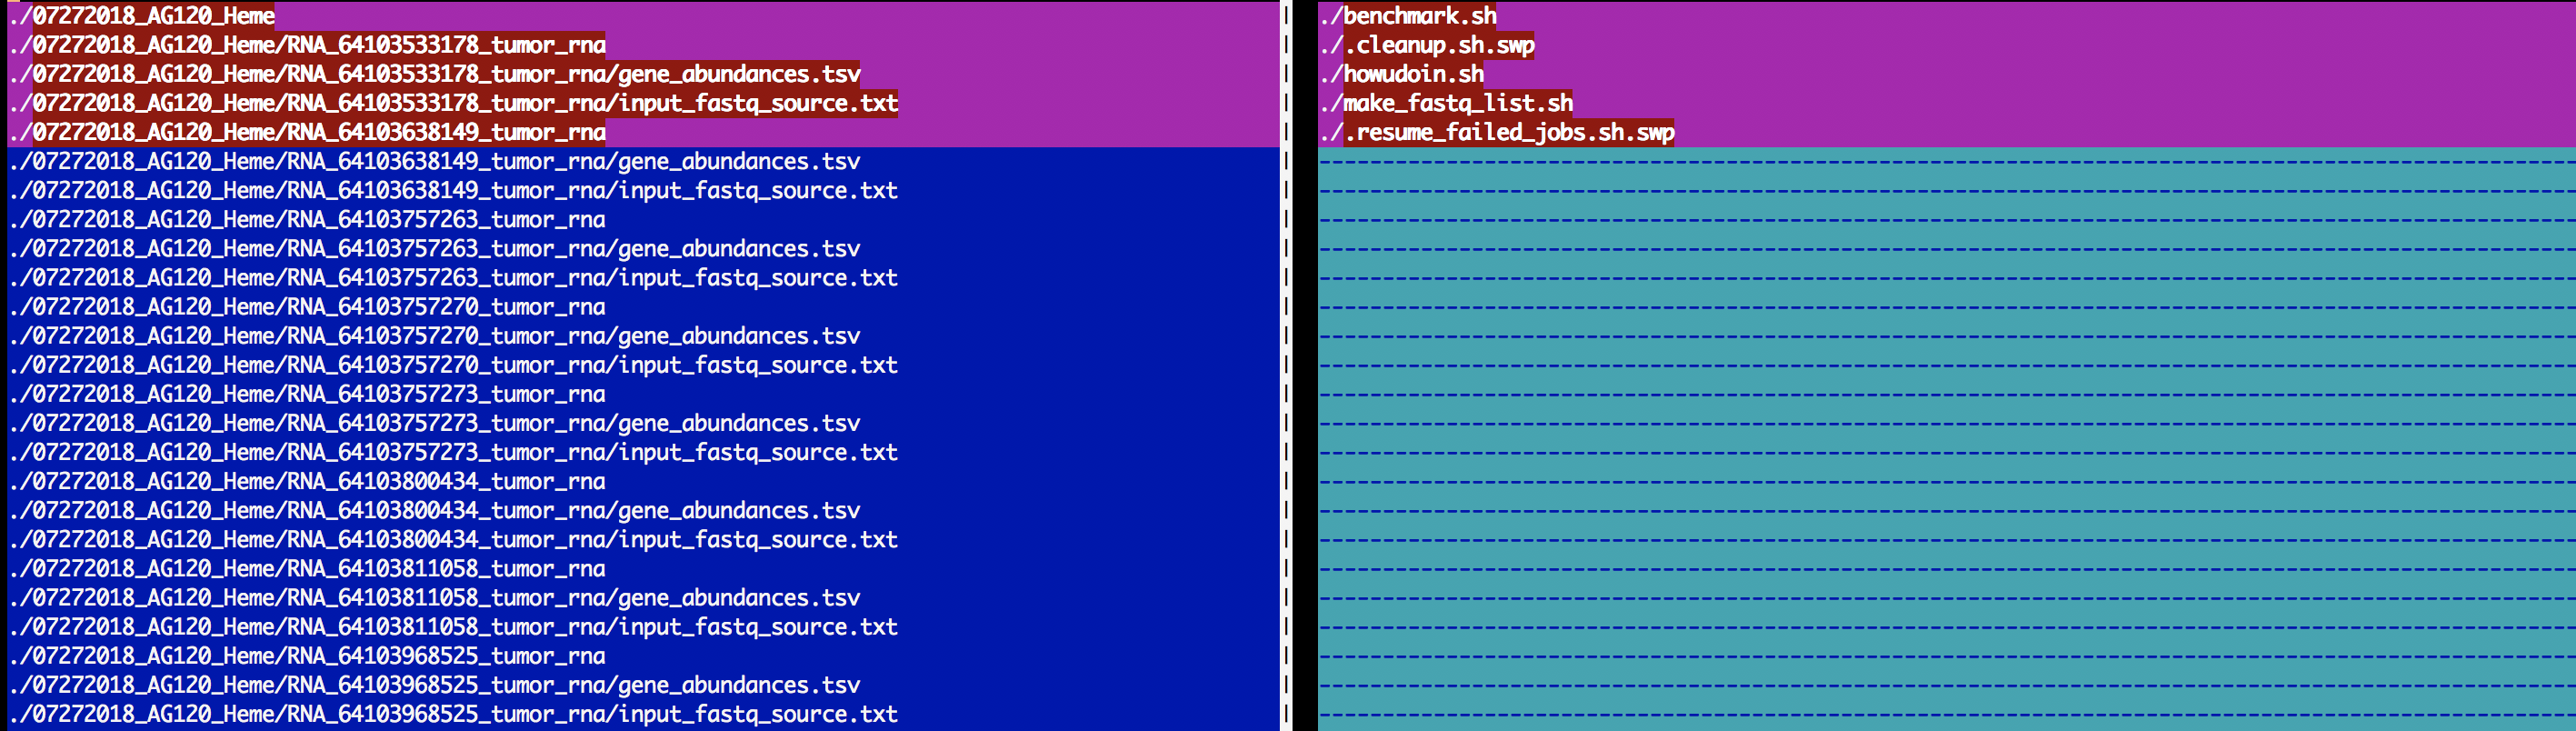
\includegraphics[width=39.36in]{images/vimdiff}

\hypertarget{sun-grid-engine}{%
\subsection{Sun Grid Engine}\label{sun-grid-engine}}

\hypertarget{deprioritize-jobs-queued-on-sge}{%
\subsubsection{Deprioritize jobs queued on SGE}\label{deprioritize-jobs-queued-on-sge}}

\begin{Shaded}
\begin{Highlighting}[]
\ExtensionTok{qalter}\NormalTok{ -p -100 }\DataTypeTok{\{jobid1..jobidn\}}
\end{Highlighting}
\end{Shaded}

\hypertarget{vim}{%
\subsection{vim}\label{vim}}

\hypertarget{repeat-content-of-line-in-new-column}{%
\subsubsection{Repeat content of line in new column}\label{repeat-content-of-line-in-new-column}}

\begin{verbatim}
# repeat content of line
# a
# b
# c
# becomes
# a = C.a
# b = C.b
# c = C.c
:%s/.*/& = C.&
\end{verbatim}

\hypertarget{r-1}{%
\section{R}\label{r-1}}

\hypertarget{heatmaps}{%
\subsection{Heatmaps}\label{heatmaps}}

\hypertarget{addition}{%
\subsection{Addition}\label{addition}}

\begin{Shaded}
\begin{Highlighting}[]
\NormalTok{x <-}\StringTok{ }\DecValTok{3}
\NormalTok{y <-}\StringTok{ }\DecValTok{4}
\NormalTok{z <-}\StringTok{ }\NormalTok{x}\OperatorTok{+}\NormalTok{y}
\NormalTok{z}
\end{Highlighting}
\end{Shaded}

\begin{verbatim}
## [1] 7
\end{verbatim}

\hypertarget{python}{%
\section{python}\label{python}}

\hypertarget{perl}{%
\section{perl}\label{perl}}

\hypertarget{get-number-of-lines-in-a-file}{%
\subsubsection{Get number of lines in a file}\label{get-number-of-lines-in-a-file}}

\begin{Shaded}
\begin{Highlighting}[]
\FunctionTok{open}\NormalTok{(}\KeywordTok{my} \DataTypeTok{$input}\NormalTok{, }\KeywordTok{"}\StringTok{-|}\KeywordTok{"}\NormalTok{, }\KeywordTok{"}\StringTok{wc -l < }\DataTypeTok{$fastqs}\KeywordTok{"}\NormalTok{);}
\KeywordTok{my} \DataTypeTok{$rc}\NormalTok{ = <}\DataTypeTok{$input}\NormalTok{>;}
\KeywordTok{if}\NormalTok{ (}\DataTypeTok{$rc}\NormalTok{ =~ }\KeywordTok{/}\CharTok{(}\BaseNTok{\textbackslash{}d}\CharTok{+)}\KeywordTok{/}\NormalTok{) \{}
    \FunctionTok{print} \DataTypeTok{$rc}\NormalTok{;}
\NormalTok{\}}
\end{Highlighting}
\end{Shaded}

\bibliography{book.bib,packages.bib}


\end{document}
